% English-to-Khmer Phonetic Transliteration: Models, Data and Human Acceptability Evaluation
% Two-column layout. Build: see README.md (XeLaTeX or LuaLaTeX, then BibTeX). Numbers come from generated/values.tex,
% which tools/extract.py writes from the project's committed result files.
\documentclass[10pt,a4paper,twocolumn]{article}

\usepackage{iftex}
\usepackage{fontspec}
\usepackage[margin=0.75in,columnsep=0.3in]{geometry}
\usepackage{microtype}
\usepackage{amsmath}
\usepackage{booktabs}
\usepackage{tabularx}
\usepackage{array}
\usepackage{multirow}
\usepackage{xcolor}
\usepackage{caption}
\usepackage{float}
\usepackage{enumitem}
\usepackage{tikz}
\usetikzlibrary{positioning,arrows.meta}
\usepackage{pgfplots}
\usepackage{pgfplotstable}
\usepgfplotslibrary{groupplots}
\pgfplotsset{compat=1.18}
\usepackage[numbers,sort&compress]{natbib}
\usepackage[hidelinks]{hyperref}
\usepackage{url}

% Khmer: Noto Serif Khmer, shaped by HarfBuzz (XeTeX shapes natively; LuaTeX needs the HarfBuzz renderer)
\ifLuaTeX
  \newfontfamily\khmerfont{Noto Serif Khmer}[Script=Khmer,Renderer=HarfBuzz,Scale=MatchLowercase]
\else
  \newfontfamily\khmerfont{Noto Serif Khmer}[Script=Khmer,Scale=MatchLowercase]
\fi
\newcommand{\km}[1]{{\khmerfont #1}}

% generated by tools/extract.py from data/results_extract.json; do not edit
\makeatletter
\@namedef{val@s.primary.acc}{16.7}
\@namedef{val@s.primary.n}{165}
\@namedef{val@s.primary.top4}{40.4}
\@namedef{val@s.primary.cer}{0.353}
\@namedef{val@s.proxy.acc}{30.1}
\@namedef{val@s.proxy.top4}{51.3}
\@namedef{val@s.proxy.n}{400}
\@namedef{val@e02.phones}{+1.6}
\@namedef{val@e02.phones.ci}{[−1.6, +4.9]}
\@namedef{val@e02.families}{162}
\@namedef{val@s.t1.p50}{17}
\@namedef{val@s.t1.p95}{30}
\@namedef{val@s.t1.load}{0.15}
\@namedef{val@s.t1.peak}{65}
\@namedef{val@s.t1.b16}{13}
\@namedef{val@s.t2.p50}{19}
\@namedef{val@s.t2.p95}{34}
\@namedef{val@s.t2.load}{0.15}
\@namedef{val@s.t2.peak}{64}
\@namedef{val@s.t2.b16}{13}
\@namedef{val@s.t3.p50}{19}
\@namedef{val@s.t3.p95}{38}
\@namedef{val@s.t3.load}{0.16}
\@namedef{val@s.t3.peak}{65}
\@namedef{val@s.t3.b16}{13}
\@namedef{val@sens.s0.donor}{36.2}
\@namedef{val@sens.s0.nopron}{32.6}
\@namedef{val@sens.s1.donor}{33.0}
\@namedef{val@sens.s1.nopron}{26.3}
\@namedef{val@sens.s2.donor}{44.7}
\@namedef{val@sens.s2.nopron}{35.8}
\@namedef{val@sens.letters.donor}{0.0}
\@namedef{val@e03.phones}{+0.6}
\@namedef{val@e03.phones.ci}{[−2.4, +3.8]}
\@namedef{val@e04.gp}{+2.2}
\@namedef{val@e04.gp.ci}{[−1.5, +6.0]}
\@namedef{val@e04.p}{−8.0}
\@namedef{val@e04.p.ci}{[−14.6, −1.4]}
\@namedef{val@e05.gp_g8}{+1.6}
\@namedef{val@e05.gp_g8.ci}{[−1.1, +4.5]}
\@namedef{val@e05.gp_gg}{+0.8}
\@namedef{val@e05.gp_gg.ci}{[−2.3, +3.9]}
\@namedef{val@e13.dev}{+1.6}
\@namedef{val@e13.dev.ci}{[−2.4, +5.6]}
\@namedef{val@e13.eval}{−1.3}
\@namedef{val@e13.eval.ci}{[−4.8, +2.3]}
\@namedef{val@e13.mech.missing}{7.1}
\@namedef{val@e13.mech.wrong}{7.9}
\@namedef{val@e13.mech.coll.missing}{10.0}
\@namedef{val@e13.mech.coll.wrong}{15.0}
\@namedef{val@e07.vs_g}{+5.8}
\@namedef{val@e07.vs_g.ci}{[+0.05, +11.6]}
\@namedef{val@e08.vs_e07}{+0.3}
\@namedef{val@e08.vs_e07.ci}{[−5.7, +6.5]}
\@namedef{val@e08.vs_e07.greedy}{+2.6}
\@namedef{val@e08.vs_e07.greedy.ci}{[−2.4, +7.5]}
\@namedef{val@e09.e08.sel_vs_reg}{+5.9}
\@namedef{val@e09.e08.sel_vs_reg.ci}{[+1.4, +10.4]}
\@namedef{val@e09.e08.greedy_vs_reg}{+5.0}
\@namedef{val@e09.e08.greedy_vs_reg.ci}{[0.0, +9.9]}
\@namedef{val@e09.e08.sel_vs_greedy}{+0.9}
\@namedef{val@e09.e08.sel_vs_greedy.ci}{[−1.4, +3.6]}
\@namedef{val@h.e07.top1}{49.9}
\@namedef{val@h.e07.cer}{0.178}
\@namedef{val@h.e08.top1}{52.4}
\@namedef{val@h.e08.cer}{0.161}
\@namedef{val@h.e11.top1}{52.3}
\@namedef{val@h.e11.cer}{0.163}
\@namedef{val@h.e12.top1}{53.0}
\@namedef{val@h.e13.top1}{51.1}
\@namedef{val@h.items}{228}
\@namedef{val@h.families}{222}
\@namedef{val@d.items}{253}
\@namedef{val@d.e11.top1}{53.0}
\@namedef{val@e11.vs_e07}{+2.5}
\@namedef{val@e11.vs_e07.ci}{[−2.7, +7.7]}
\@namedef{val@e11.vs_e08}{−0.1}
\@namedef{val@e11.vs_e08.ci}{[−4.7, +4.6]}
\@namedef{val@e12.vs_e11.hist}{+0.7}
\@namedef{val@e12.vs_e11.hist.ci}{[−4.1, +5.4]}
\@namedef{val@e11.update}{3,000}
\@namedef{val@e11.sha}{286292a4f21131d0dd238d48919485192b0b0eb268d005bbc804d3ff78229713}
\@namedef{val@e12.update}{6,000}
\@namedef{val@e13.update}{800}
\@namedef{val@rev.representative.e07}{24}
\@namedef{val@rev.representative.e08}{30}
\@namedef{val@rev.representative.e11}{29}
\@namedef{val@rev.disagreement.e07}{5}
\@namedef{val@rev.disagreement.e08}{8}
\@namedef{val@rev.disagreement.e11}{10}
\@namedef{val@t1.e11.acceptable}{77}
\@namedef{val@t1.e11.not_acceptable}{40}
\@namedef{val@t1.e11.uncertain}{3}
\@namedef{val@t1.e11.share}{64.2}
\@namedef{val@t1.e12.acceptable}{77}
\@namedef{val@t1.e12.not_acceptable}{39}
\@namedef{val@t1.e12.uncertain}{4}
\@namedef{val@t1.e12.share}{64.2}
\@namedef{val@t1.diff}{0.0}
\@namedef{val@t1.diff.ci}{[−8.3, +8.3]}
\@namedef{val@t1.paired.both}{63}
\@namedef{val@t1.paired.a_only}{14}
\@namedef{val@t1.paired.b_only}{14}
\@namedef{val@t1.paired.neither}{29}
\@namedef{val@t1.p}{1.00}
\@namedef{val@t2.e11.acceptable}{90}
\@namedef{val@t2.e11.not_acceptable}{29}
\@namedef{val@t2.e11.uncertain}{1}
\@namedef{val@t2.e11.share}{75.0}
\@namedef{val@t2.e13.acceptable}{90}
\@namedef{val@t2.e13.not_acceptable}{29}
\@namedef{val@t2.e13.uncertain}{1}
\@namedef{val@t2.e13.share}{75.0}
\@namedef{val@t2.diff}{0.0}
\@namedef{val@t2.diff.ci}{[−7.5, +7.5]}
\@namedef{val@t2.paired.both}{79}
\@namedef{val@t2.paired.a_only}{11}
\@namedef{val@t2.paired.b_only}{11}
\@namedef{val@t2.paired.neither}{19}
\@namedef{val@t2.p}{1.00}
\@namedef{val@t2.ordinary.e11}{34}
\@namedef{val@t2.ordinary.e13}{32}
\@namedef{val@t2.irregular.e11}{20}
\@namedef{val@t2.irregular.e13}{21}
\@namedef{val@t2.names.e11}{36}
\@namedef{val@t2.names.e13}{37}
\@namedef{val@t1.ordinary.e12}{27}
\@namedef{val@t1.ordinary.e11}{27}
\@namedef{val@t1.irregular.e12}{19}
\@namedef{val@t1.irregular.e11}{14}
\@namedef{val@t1.names.e12}{31}
\@namedef{val@t1.names.e11}{36}
\@namedef{val@cov.words}{23}
\@namedef{val@cov.greedy}{8}
\@namedef{val@cov.beam1}{10}
\@namedef{val@cov.any4}{15}
\@namedef{val@cov.any5}{15}
\@namedef{val@cov.recov}{7}
\@namedef{val@cov.none}{8}
\@namedef{val@cov.cands}{93}
\@namedef{val@cov.unc}{6}
\@namedef{val@cov.coverage}{100.0}
\@namedef{val@cov.gain_vs_greedy}{7}
\@namedef{val@cov.gain_vs_beam1}{5}
\@namedef{val@par.dev}{0}
\@namedef{val@par.dev.n}{276}
\@namedef{val@par.eval}{0}
\@namedef{val@par.eval.n}{245}
\@namedef{val@par.top4}{0}
\@namedef{val@b.lat1}{554}
\@namedef{val@b.lat4}{820}
\@namedef{val@b.load}{7.1}
\@namedef{val@b.peak}{2019}
\@namedef{val@b.rss}{713}
\@namedef{val@b.wps}{14.5}
\@namedef{val@b.i.load}{5.5}
\@namedef{val@b.i.wps}{14.1}
\@namedef{val@b.i.par}{0}
\@namedef{val@b.i.checks}{True}
\@namedef{val@b.i.nchecks}{19}
\newcommand{\val}[1]{\@ifundefined{val@#1}{\textbf{??#1}}{\@nameuse{val@#1}}}
\makeatother


\captionsetup{font=small,labelfont=bf,skip=4pt}
\setlength{\emergencystretch}{2em}
\renewcommand{\bibfont}{\small\raggedright}
\setlist{itemsep=1pt,topsep=3pt}
\newcolumntype{L}{>{\raggedright\arraybackslash}X}
\newcommand{\pp}{\,pp}

\title{English-to-Khmer Phonetic Transliteration:\\ Models, Data and Human Acceptability Evaluation}
\author{Richard Cheam\\ \small \href{mailto:richardcheam912@gmail.com}{\texttt{richardcheam912@gmail.com}}}
\date{Technical report, 31 October 2026}

\hypersetup{pdftitle={English-to-Khmer Phonetic Transliteration: Models, Data and Human Acceptability Evaluation},
  pdfauthor={Richard Cheam}}

\begin{document}
\maketitle

\begin{abstract}
\noindent
We study a narrow task: given one English word or name, write in Khmer script how it sounds when read in English.
Two systems are released as research previews: a 2.6M-parameter character-level Transformer trained from scratch,
and a LoRA adapter for ByT5-small. Both are trained on English--Khmer pairs mined from bracketed web text, the
adapter additionally on spellings attested in the ALT Parallel Corpus; no LLM-generated labels are used in either
released model. Early experiments scored models by exact agreement with single mined or curated reference
spellings. A blinded review later showed that such agreement both rejects acceptable alternatives and accepts
unwanted spellings, so the final evaluation uses blinded acceptable/not acceptable/uncertain judgments by a single
project-affiliated judge on prospectively frozen samples of 120 word families. On two such samples the released
adapter's spelling was judged acceptable for \val{t1.e11.share}\% and \val{t2.e11.share}\% of words; a longer
training schedule and pronunciation-guided training each left acceptability unchanged on their own sample
(differences \val{t1.diff}\pp{} and \val{t2.diff}\pp). Adding English pronunciation input produced no detectable change in reference agreement in four experiments,
although the intervals do not exclude gains of a few points. Irregularly spelled words remain the weakest group,
and in a small diagnostic, alternative beam candidates often contained an acceptable spelling that greedy decoding
missed.
\end{abstract}

% =====================================================================================================
\section{Introduction and task}
\label{sec:intro}

A Khmer text-to-speech front-end receives English words inside Khmer text---names, product terms, loanwords---and
needs them in Khmer script before a Khmer-only speech model can read them. This report documents a transliterator
for that step. Its input is one English word or name; its output is a Khmer-script spelling that a Khmer reader
would pronounce close to the word's \emph{English} pronunciation. For example, the released adapter writes
\emph{coffee} as \km{ខូហ្វី} and \emph{london} as \km{ឡុនដុន}.

The task differs from three neighbouring ones.
It is not \emph{translation}: meaning is ignored.
It is not \emph{romanised-Khmer conversion}, where Latin letters encode a Khmer word (\emph{sok sabay}).
And it is not reproducing \emph{established loan spellings} regardless of pronunciation: the usual Khmer form of
\emph{coffee} is \km{កាហ្វេ}, which does not follow the English pronunciation; the task's target does.

Three properties make the task hard to measure. First, English spelling underdetermines pronunciation
(\emph{record}, \emph{live}, irregular names), so a target requires a declared reading; this project uses the first
General American reading in CMUdict \citep{cmudict}. Second, Khmer adaptation is many-to-one and one-to-many: the
script has two consonant series, inherent vowels, subscript consonants and series-shifting diacritics
(as in \km{ម៉} and \km{ប៊}), so several spellings can render the same sound acceptably. Third, the available supervision is
web text written by many people under different conventions.

The contributions are proportionate to a small project:
(i) two implemented and released systems with a common command-line and Python interface;
(ii) a documented data pipeline, including the repair of a selection error that silently removed dictionary-word
targets;
(iii) a set of controlled comparisons of pronunciation input, data, schedule and decoding, each registered before
its results were seen; and
(iv) a human-acceptability evaluation protocol with frozen inputs, blinded spellings and explicit labels. No new
architecture or general benchmark is claimed.

% =====================================================================================================
\section{Related work}
\label{sec:related}

\paragraph{Grapheme, phoneme and hybrid transliteration.}
\citet{oh-choi-2005-ensemble} distinguish grapheme-based, phoneme-based and hybrid models for English--Korean and
English--Japanese transliteration and report gains from combining source graphemes and phonemes dynamically.
\citet{ngo-etal-2015-phonology} model target-language phonology explicitly for low-resource transliteration into
Vietnamese, motivated by phonologically invalid outputs. These works motivate the project's \emph{hypothesis} that
supplying CMUdict phones would help; whether it does for Khmer with small mined data is what
Section~\ref{sec:res-pron} tests.

\paragraph{Byte-level pretrained models.}
ByT5 \citep{xue-etal-2022-byt5} operates on UTF-8 bytes and is reported to be more robust to noise and stronger on
spelling- and pronunciation-sensitive tasks than token-based counterparts. \citet{kirov-etal-2024-context} fine-tune
ByT5 for single-word transliteration of romanised South Asian languages and find its fine-tuning sensitive to noisy
training items: removing the 10\% least representative pairs helped, while non-pretrained models did not benefit.
The adapter released here uses ByT5-small with LoRA \citep{hu-etal-2022-lora}. Khmer characters are three UTF-8
bytes each, a detail that matters for adaptation (Section~\ref{sec:models}).

\paragraph{Evaluation with multiple references.}
The NEWS 2018 shared task \citep{chen-etal-2018-news} scores transliteration against reference \emph{lists}, where
any listed variant counts (ACC), alongside mean F-score, MRR and MAP. This project has one mined spelling per item
for most of its history, so only exact agreement and character error rate are computed against it; the human
evaluation instead judges each produced spelling, which admits any number of acceptable variants.

\paragraph{Candidate generation and rescoring.}
\citet{grundkiewicz-heafield-2018-neural} apply NMT techniques to named-entity transliteration, including
ensembling and rescoring n-best lists with right-to-left models. Rescoring can only help when acceptable spellings
are already in the candidate list; Section~\ref{sec:res-rank} measures that presence for the released adapter. No
reranker is built here.

% =====================================================================================================
\section{Data and models}
\label{sec:data}

\subsection{Mined pairs and the selection repair}

Training pairs come from Khmer web text in which a Khmer spelling is followed by the English word in brackets, e.g.
``\km{ចនសុន} (Johnson)'', mined from the Khmer subset of FineWeb-2 \citep{penedo-etal-2025-fineweb2,fineweb2-card}
and a Khmer Wikipedia dump of 2026-10-01 \citep{wikimedia-tou}. A pair is kept when the English word is in CMUdict,
passes a noise filter, does not look like romanised Khmer, and belongs to no word family used for evaluation. A
\emph{family} groups an English word with its plurals and other inflections; exclusion and bootstrap resampling both
operate on families so that \emph{band} and \emph{bands} cannot fall on opposite sides of a split.

The original miner labelled a pair \texttt{khmer\_like}, and dropped it, if its Latin side was a known romanised
Khmer word \emph{or} its Khmer side was a known Khmer word. The second condition removed exactly the pairs whose
Khmer spelling is in the Google Khmer lexicon \citep{google-langres-km}, including established loans; a later
diagnostic found 0 of 10,031 training targets covered by exact lexicon lookup, by construction. Separating the two
conditions recovered 11,377 rows; romanised-Latin rows stayed excluded.

\paragraph{Consonant screening and its limits.}
To check that a mined spelling plausibly renders the English word, a rule-based reader maps Khmer consonants to
sound classes and compares them with the CMUdict reading. On 30,980 held-out lexicon headwords its consonant classes
agreed with the lexicon's own transcriptions for 88.6\%. The screen does not read vowels at all. After the repair,
2,967 dictionary-assessable, consonant-screened pairs remained. A later audit recovered 1,292 pairs that the
screen had rejected because of documented weaknesses (for example doubled letters and glides), and added 1,217
names and loanwords whose Khmer spelling occurs verbatim in the human translations of the ALT Parallel Corpus
\citep{riza-etal-2016-alt,nict-alt}, passed through the same screen. None of these spellings was reviewed by a
person, and vowel quality is unassessed throughout.

\paragraph{Synthetic labels (historical only).}
One data-expansion experiment added 384 rows for 193 words whose spellings were suggested by Google's AI
Mode. They were
used only in historical runs. The released adapter's training file contains none (verified row by row), and the
released small model never used them.

\subsection{The two released models}
\label{sec:models}

Table~\ref{tab:releases} summarises the releases.

\paragraph{Small character-level Transformer.}
An encoder--decoder with $d_\text{model}=192$, three encoder and three decoder layers, four heads and feed-forward
width 512 (2.6M parameters), trained from scratch on 9,735 mined pairs (296 more held out for validation loss) with
AdamW, learning rate $10^{-3}$, cosine decay and label smoothing 0.1. The epoch (27 of 40) was selected on 86
development items; final scores come from separate test items. Inference runs in NumPy with beam search of width 4.
The released weights are the letters-only seed-0 run (\texttt{letters\_s0}); the file on the Hub is byte-identical
to the recorded checkpoint (sha256 \texttt{8901050b\ldots}).

\paragraph{ByT5-small with a LoRA adapter.}
The base \texttt{google/byt5-small} (revision \texttt{68377bdc}) is frozen. LoRA matrices of rank 16 and
$\alpha=32$ are added to every attention projection (q, k, v, o) and gated feed-forward layer (wi\_0, wi\_1, wo):
256 tensors, 6.26M parameters. Training used 4,764 pairs over 3,585 words---2,255 screened mined pairs, 1,292
recovered pairs and 1,217 ALT-attested pairs---with AdamW at $10^{-3}$, 100 warm-up steps then linear decay,
batch 32 and \val{e11.update} updates (4.6 hours on six CPU threads, one seed). Checkpoints were selected by
greedy exact agreement on 253 development items, then CER. The selected checkpoint was the last one evaluated;
that alone does not show the model was under-trained, and a twice-longer schedule did not change acceptability
(Section~\ref{sec:res-train}).

An earlier ByT5 attempt with attention-only adapters and 1,000 updates produced nearly the same output for
every input (\km{ហ្វេន} for 204 of 228 evaluation words). A diagnosis found no pipeline bug: two of the three
UTF-8 bytes of a Khmer character are almost free to predict, so a falling per-byte loss coexisted with an
input-independent letter model. Adding feed-forward adapters and training longer produced an input-dependent model;
which change mattered was not isolated.

The adapter is stored in a project format (\texttt{adapter.safetensors} with keys ending in \texttt{.A}/\texttt{.B}
plus a JSON configuration), not as a PEFT checkpoint. It loads only through the package's \texttt{khmer\_translit.byt5}
module, which wraps the base model's linear layers and refuses a base whose revision or weight hash differs from the
pinned one. Single answers use greedy decoding; candidate lists use beam search with
\texttt{early\_stopping="never"} and no length penalty (Section~\ref{sec:res-decode}).

\begin{table*}[t]
\centering\small
\caption{The two released systems. Latency and memory: Intel Core i7-8750H laptop, CPU only; the small model's
latency is the range of three recorded runs.}
\label{tab:releases}
\begin{tabularx}{\textwidth}{@{}lLL@{}}
\toprule
 & Small Transformer & ByT5-small + LoRA adapter \\
\midrule
Repository & \texttt{ric912/en-km-phonetic-}\newline\texttt{transliterator} (tag v0.2.0) &
  \texttt{ric912/en-km-phonetic-byt5-lora} \\
Parameters & 2.6M, trained from scratch & 300M frozen base + 6.26M adapter \\
Training pairs & 9,735 mined (FineWeb-2, Wikipedia) & 4,764 (mined, recovered, ALT-attested) \\
Runtime & NumPy only & PyTorch, Transformers, safetensors; base fetched separately (1.2\,GB) \\
Decoding & beam 4 & greedy; beam $\ge 4$ for candidates \\
Load time & \val{s.t1.load}--\val{s.t3.load}\,s & \val{b.i.load}--\val{b.load}\,s \\
One word (median) & \val{s.t1.p50}--\val{s.t3.p50}\,ms & \val{b.lat1}\,ms (greedy), \val{b.lat4}\,ms (top-4) \\
Batched & \val{s.t1.b16}\,ms per word (batches of 16) & \val{b.wps} words/s (greedy) \\
Peak memory & \val{s.t1.peak}\,MiB & \val{b.peak}\,MB \\
Weights licence & CC BY-NC-SA 4.0 & CC BY-NC-SA 4.0 (base: Apache 2.0) \\
\bottomrule
\end{tabularx}
\end{table*}

\paragraph{Data separation.}
For each experiment, training, validation, checkpoint selection and evaluation used disjoint families. The small
model's final references were opened once, after all seven of its comparison runs were frozen. The adapter
experiments share a \emph{historical} development set (253 items) and evaluation set (228 items, 222 families) that
were examined repeatedly across eleven experiments; scores on them are exploratory. The human tests (Section~\ref{sec:eval})
used fresh families excluded from all training files. The two released models were trained on different data and
were never evaluated on a common, clean test set: the historical evaluation set overlaps the small model's training
words (122 of its words have other targets there), so no head-to-head comparison is reported.

% =====================================================================================================
\section{Evaluation methodology}
\label{sec:eval}

\paragraph{Reference agreement.}
Early experiments scored the top output against one reference spelling per item: exact agreement, averaged over
families, and character error rate (CER). For the small model the references were a curated list of 165 items in
162 families (spellings checked by the author, with 94 items chosen from an earlier model's candidates) and an
exploratory list of 400 LLM-suggested, spot-checked spellings. For the adapters they were the mined spellings
themselves. Agreement is not phonetic accuracy: one acceptable spelling per item cannot admit legitimate variants,
and an unreviewed reference can itself be wrong.

\paragraph{Intervals.}
Paired differences between two systems use a family-level bootstrap with 10,000 resamples. These intervals are
\emph{conditional} on the trained checkpoints: they describe item sampling, not training-seed variation, and
exclude the extra uncertainty of checkpoint selection. Where three paired seeds exist, their per-seed differences
are reported as well. Intervals for differences are not intervals for either model's own rate, and a difference
whose interval includes zero is not evidence of equivalence.

\paragraph{Human acceptability.}
A spelling is \emph{acceptable} if a Khmer reader would pronounce it close to the declared General American
reading, \emph{not acceptable} otherwise, and \emph{uncertain} when the judge cannot decide; the policy file was
fixed before the reviews and unchanged across them. The judge is the project's author---a single,
project-affiliated judge. Spellings were shown on a local page without model identity, rank or score, with labels
in seeded random order; identical spellings from two systems were shown once. Every spelling required an explicit
click; unanswered spellings are \emph{missing}, never counted as rejections, and an unjudged spelling stays
unassessed.

Two sampling designs were used and are never pooled. A development review of 60 words used a representative sample of 40 words and an
enriched sample of 20 words where the compared systems disagreed, reported separately; its labels were
given in chat and transcribed under rules the judge confirmed. Two prospective tests then each drew 120 fresh
families---40 ordinary words, 40 irregular spellings and 40 names---frozen before the candidate model was trained,
with all predictions frozen before review. ``Confirmed acceptable'' counts uncertain as not acceptable; sensitivity
analyses recount uncertain both ways. These judgments are useful task-specific evidence of acceptability for this
judge and policy; they are not independent, and the 40/40/40 design does not estimate performance on everyday text.

% =====================================================================================================
\section{Results}
\label{sec:results}

Table~\ref{tab:comparisons} lists the principal comparisons; Table~\ref{tab:tests} gives the blinded tests.

\begin{table*}[t]
\centering\small
\caption{Principal comparisons. $\Delta$ is in percentage points with a 95\% paired family-bootstrap interval,
conditional on the checkpoints. Reference agreement is exploratory except where marked.}
\label{tab:comparisons}
\begin{tabularx}{\textwidth}{@{}>{\raggedright\arraybackslash}p{2.3cm}L>{\raggedright\arraybackslash}p{3.3cm}>{\raggedright\arraybackslash}p{4.1cm}@{}}
\toprule
Question & Comparison (experiment) & $\Delta$ [95\%] & Evidence and limits \\
\midrule
Pronunciation input & small model, letters + phones vs letters (E02) & \val{e02.phones} \val{e02.phones.ci} &
  curated references, 162 families; 3 paired seeds, all positive; registered, inconclusive \\
 & same, on consonant-screened pairs (E03) & \val{e03.phones} \val{e03.phones.ci} & mined references; 3 seeds \\
 & letters + phones vs letters (E04) & \val{e04.gp} \val{e04.gp.ci} & mined references; 3 seeds \\
 & pooled letters+phones candidates vs letters top-8 (E05) & \val{e05.gp_g8} \val{e05.gp_g8.ci} &
  top-8 oracle, equal budget \\
 & adapter with CMUdict reading vs released adapter (E13) & \val{e13.eval} \val{e13.eval.ci} &
  mined references; several ingredients changed \\
\midrule
ByT5 adaptation & corrected adapter vs mean of 3 small letters models (E07) & \val{e07.vs_g} \val{e07.vs_g.ci} &
  registered beam-4; one adapter run \\
\midrule
More data & + recovered, ALT and synthetic rows vs screened mined pairs only (E08 vs E07) & \val{e08.vs_e07} \val{e08.vs_e07.ci} &
  registered beam-4; greedy \val{e08.vs_e07.greedy} \val{e08.vs_e07.greedy.ci} \\
 & real data only vs E07, greedy (E11 vs E07) & \val{e11.vs_e07} \val{e11.vs_e07.ci} & one run each \\
 & real data only vs with synthetic rows (E11 vs E08) & \val{e11.vs_e08} \val{e11.vs_e08.ci} & one run each \\
\midrule
Longer training & 6,000 vs 3,000 updates (E12 vs E11) & \val{e12.vs_e11.hist} \val{e12.vs_e11.hist.ci} &
  one seed; blinded test in Table~\ref{tab:tests} \\
\bottomrule
\end{tabularx}
\end{table*}

\subsection{Did pronunciation input help?}
\label{sec:res-pron}

No experiment detected a benefit. In the small model's registered comparison, adding CMUdict phones next to the
letters changed curated-reference agreement by \val{e02.phones}\pp{} on average over three paired seeds (per seed
$+0.6$, $+1.5$, $+2.8$), with interval \val{e02.phones.ci}. The interval excludes the registered 5-point threshold
and includes zero; with an estimated power of 0.29 for a true 5-point gain, the result is inconclusive, not null.
Repeating the comparison on dictionary-assessable, consonant-screened pairs and with a phones-only arm gave the
same picture (Table~\ref{tab:comparisons}); a phones-only model scored \val{e04.p}\pp{} against letters (one seed) but got different
words right, and pooling the two models' candidates did not beat a letters model's own top-8 list at equal budget.

Sensitivity diagnostics explain part of this. Supplying another word's phones changed the small model's top output
for \val{sens.s0.donor}--\val{sens.s2.donor}\% of 94 words, depending on the seed, but the changed outputs moved
toward the donor's consonants in only 2--7 cases per seed; most changes were vowel or diacritic edits, and
letters-only controls, as intended, never changed. The pronunciation-guided adapter behaved similarly:
removing the reading changed \val{e13.mech.missing}\% of historical-development outputs and a wrong reading
\val{e13.mech.wrong}\%. These diagnostics show weak dependence on the supplied phones in these models and data; they
do not show that pronunciation information cannot help Khmer transliteration.

\subsection{Did more real data help?}
Recovering screened-out pairs and adding ALT-attested spellings roughly doubled the adapter's data. Against the
first corrected adapter, the released real-data adapter's greedy agreement on the historical evaluation set was
\val{h.e11.top1}\% vs \val{h.e07.top1}\% (\val{e11.vs_e07}\pp, \val{e11.vs_e07.ci}), and a version that also
used the synthetic labels was indistinguishable (\val{e11.vs_e08}\pp). Reference agreement could not separate these
models. The blinded development review could: the real-data adapter's greedy spelling was acceptable for
\val{rev.representative.e11} of 40 representative words against \val{rev.representative.e07} for the first corrected
adapter, and for \val{rev.disagreement.e11} of 20 disagreement words against \val{rev.disagreement.e07}; the
synthetic-label version scored \val{rev.representative.e08} and \val{rev.disagreement.e08}. This was a post hoc
development review with one judge, not a registered test.

\subsection{Did longer training help?}
\label{sec:res-train}
Doubling the schedule to 6,000 updates changed 65 of 120 test spellings without changing how many were
acceptable: \val{t1.e12.acceptable} vs \val{t1.e11.acceptable} of 120 (\val{t1.diff}\pp, \val{t1.diff.ci};
\val{t1.paired.a_only} vs \val{t1.paired.b_only} discordant words, exact $p=\val{t1.p}$). Historical agreement
moved by \val{e12.vs_e11.hist}\pp. One seed was run, so a small effect is not excluded.

\subsection{How did decoding configuration affect results?}
\label{sec:res-decode}
For the adapters, greedy decoding had beaten the registered beam-4 search. An inference-only audit traced
this to \texttt{early\_stopping=True}: at the byte level, junk hypotheses (an immediate end symbol, or one letter
and an end symbol) finish within the first steps and fill the beam's finished set before real spellings end.
Registered beam-4 kept only 3.60 distinct candidates per item for the synthetic-data adapter and often dropped the series-shifting diacritics (\emph{mani}
\km{ម៉ានី} became \km{មានី}). With \texttt{early\_stopping="never"}, beam top-1 was about as good as greedy
(\val{e09.e08.sel_vs_greedy}\pp, \val{e09.e08.sel_vs_greedy.ci}) and \val{e09.e08.sel_vs_reg}\pp{}
\val{e09.e08.sel_vs_reg.ci} above the registered beam on the historical evaluation set. Earlier ByT5 comparisons that used the
registered beam are therefore shifted; this report quotes greedy figures for adapters where they exist.

\subsection{How does reference agreement differ from acceptability?}
In the development review, the judge rated 109 distinct spellings. Of the 72 that differed from the mined
reference, 28 (39\%) were acceptable (for example \emph{cameroon} \km{ខេមឺរ៉ុន} and \emph{band} \km{បេន}); of
the 37 that matched it, 8 (22\%) were not acceptable (\emph{band} \km{បាន}). Exact agreement can therefore both
reject acceptable alternatives and accept unwanted spellings; it is not a one-directional underestimate.
Figure~\ref{fig:measures} shows the two kinds of evidence side by side, on separate axes because they are measured
on different items with different definitions.

\begin{figure*}[t]
\centering
\pgfplotstableread[col sep=comma]{generated/fig_reference.csv}\figref
\pgfplotstableread[col sep=comma]{generated/fig_accept.csv}\figacc
\begin{tikzpicture}
\begin{groupplot}[group style={group size=2 by 1, horizontal sep=4.25cm},
  width=4.45cm, height=4.4cm, xmin=0, xmax=100, xtick={0,25,50,75,100}, xmajorgrids, grid style={gray!25},
  tick label style={font=\scriptsize}, label style={font=\scriptsize}, title style={font=\small},
  ytick=data, yticklabel style={font=\scriptsize, align=right}, ymin=0.4]
\nextgroupplot[title={(a) Agreement with mined spellings}, xlabel={greedy exact agreement, \% (228 items)},
  yticklabels from table={\figref}{label}, ymax=5.6]
\addplot[only marks, mark=*, mark size=2pt, black] table[x=top1, y=y]{\figref};
\nextgroupplot[title={(b) Blinded acceptability}, xlabel={confirmed acceptable, \% (120 words each)},
  yticklabels from table={\figacc}{label}, ymax=6.1,
  extra y ticks={3}, extra y tick labels={}, extra y tick style={grid=major, grid style={black!60, dashed}}]
\addplot[only marks, mark=square*, mark size=2pt, black] table[x=share, y=y]{\figacc};
\node[font=\scriptsize, anchor=west, gray!60!black] at (axis cs:1,5.65) {test sample 1};
\node[font=\scriptsize, anchor=west, gray!60!black] at (axis cs:1,2.6) {test sample 2};
\end{groupplot}
\end{tikzpicture}
\caption{Two different measures, not a common benchmark. (a) Historical evaluation set, examined repeatedly,
single unreviewed reference per item. (b) Two separate prospective samples; each compares its candidate with the
released adapter on the same 120 words, and values are not comparable across samples. No uncertainty bars are drawn
for individual rates; paired differences are in Table~\ref{tab:tests}.}
\label{fig:measures}
\end{figure*}

\subsection{Is candidate ranking a plausible remaining opportunity?}
\label{sec:res-rank}
For 23 irregularly spelled development words (frozen before generation, none from test families), the judge rated
every distinct candidate among the adapter's greedy output and four canonical beam candidates
(all \val{cov.cands} distinct spellings judged; earlier judgments reused only for the identical word,
reading and spelling). The greedy output was acceptable for \val{cov.greedy} words and beam top-1 for
\val{cov.beam1}; at least one of the four beam candidates was acceptable for \val{cov.any4}. A perfect selector over
those four would add \val{cov.gain_vs_greedy} words relative to greedy and \val{cov.gain_vs_beam1} relative to beam
top-1; \val{cov.none} words had no acceptable candidate. This oracle is an upper bound for a reranker on this
sample, not achieved accuracy, and 23 hand-picked hard words cannot show whether ranking or generation is the larger
limitation in general.

\begin{table*}[t]
\centering\small
\caption{Prospective blinded tests (one judge). Each sample compares a candidate with the released adapter on its
own 120 fresh families; the two samples are different and are not pooled. Uncertain (Unc.) counts as not
confirmed. Ord.\ = ordinary words, Irreg.\ = irregular spellings. $\Delta$: candidate minus released adapter,
percentage points, 95\% paired family bootstrap.}
\label{tab:tests}
\setlength{\tabcolsep}{4pt}
\begin{tabular}{@{}llcccccc@{}}
\toprule
Sample & System & Acceptable & Unc. & Ord. & Irreg. & Names & $\Delta$ [95\%] \\
 & & of 120 & & of 40 & of 40 & of 40 & \\
\midrule
\multirow{2}{*}{1 (E12)} & Released adapter (E11) & \val{t1.e11.acceptable} (\val{t1.e11.share}\%) &
  \val{t1.e11.uncertain} & \val{t1.ordinary.e11} & \val{t1.irregular.e11} & \val{t1.names.e11} & \\
 & 6,000 updates (E12) & \val{t1.e12.acceptable} (\val{t1.e12.share}\%) & \val{t1.e12.uncertain} &
  \val{t1.ordinary.e12} & \val{t1.irregular.e12} & \val{t1.names.e12} & \val{t1.diff} \val{t1.diff.ci} \\
\midrule
\multirow{2}{*}{2 (E13)} & Released adapter (E11) & \val{t2.e11.acceptable} (\val{t2.e11.share}\%) &
  \val{t2.e11.uncertain} & \val{t2.ordinary.e11} & \val{t2.irregular.e11} & \val{t2.names.e11} & \\
 & Pronunciation-guided (E13) & \val{t2.e13.acceptable} (\val{t2.e13.share}\%) & \val{t2.e13.uncertain} &
  \val{t2.ordinary.e13} & \val{t2.irregular.e13} & \val{t2.names.e13} & \val{t2.diff} \val{t2.diff.ci} \\
\bottomrule
\end{tabular}
\end{table*}

\paragraph{Pronunciation-guided training on the second sample.}
The second test evaluated a model that changed several things at once: CMUdict readings as input, the judge's
accepted spellings of 42 difficult training families mixed into 10\% of batches, replay of the original data, and
initialisation from the released adapter. Acceptability was identical (\val{t2.e13.acceptable} vs
\val{t2.e11.acceptable}; \val{t2.paired.a_only} vs \val{t2.paired.b_only} discordant words). Because the
ingredients were not varied separately, this result cannot attribute any effect, or its absence, to one of them.
Across both samples, irregular spellings were the weakest group (\val{t1.irregular.e11}/40 and
\val{t2.irregular.e11}/40 for the released adapter).

% =====================================================================================================
\section{Released systems and reproducibility}
\label{sec:release}

Both models are published under CC BY-NC-SA 4.0 for the weights \citep{release-small,release-byt5}; the
\texttt{khmer-translit} package that runs them is under PolyForm Noncommercial 1.0.0 and its wheel is attached to
the small model's repository. The small model needs only NumPy and answers in tens of milliseconds. The adapter
needs PyTorch and Transformers and a separate download of the pinned base; it is about 30 times slower per word and
uses about 2\,GB of memory, so it suits drafting rather than high-volume use on a CPU.

Before release the adapter export was verified to be bit-identical to the training checkpoint (sha256
\texttt{286292a4\ldots}), and the packaged loader reproduced the frozen research predictions with
\val{par.dev} mismatches on \val{par.dev.n} development and \val{par.eval} on \val{par.eval.n} evaluation words
(greedy) and \val{par.top4} mismatches in top-4 lists. A fresh, isolated CPU-only installation passed all
\val{b.i.nchecks} checks with network access blocked at the socket level, including refusal of empty, multi-word,
non-Latin and over-long inputs and of corrupt or mismatched files. The published repositories were re-downloaded and
the quick-start commands re-run. Both interfaces share one command (\texttt{khmer-translit predict}); exact usage is
in each model card and in the report's companion README. Training data, judgments and references are not
distributed.

% =====================================================================================================
\section{Limitations and conclusion}
\label{sec:conclusion}

\paragraph{Limitations.}
\emph{Supervision} is mined and unreviewed; the consonant screen ignores vowels, which were the largest class of
reference disagreement for every adapter (40--50\% of mismatches). \emph{References} cover one spelling per item,
and much of the reference-based evidence comes from a historical evaluation set examined across many experiments.
\emph{Human evaluation} rests on one project-affiliated judge, samples of 120 words (each rate is uncertain by
roughly $\pm 8$ points), a 40/40/40 design that over-represents hard words and names, and one training seed per
adapter. \emph{Pronunciation policy} fixes one General American reading per word, and CMUdict coverage limits which
words can be checked. \emph{Permissions}: rights in the mined web pages remain with their authors; FineWeb-2 is
distributed under ODC-By 1.0 and Common Crawl's terms \citep{fineweb2-card}, and whether Wikipedia's share-alike
condition \citep{wikimedia-tou} extends to trained weights is legally unsettled. \emph{Scope}: single words only; sentences, context and romanised Khmer are out of scope.

\paragraph{Conclusion.}
Two English-to-Khmer phonetic transliterators are documented and released with their evidence. Within this
project's data and models, English pronunciation input, more training updates and pronunciation-guided training
produced no detectable gain, and a decoding configuration error---not model quality---explained an apparent beam
search deficit for byte-level models. The most informative measurement change was moving from single-reference
agreement to blinded acceptability judgments, which separated models that agreement could not. On two separate
120-word samples, the released adapter's spelling was judged acceptable for 64--75\% of words, and for 35--50\% of
irregularly spelled words. The candidate diagnostic indicates that acceptable alternatives are often already generated,
while about a third of the hard words had none; which of the two dominates on ordinary text remains unmeasured.

\bibliographystyle{plainnat}
\bibliography{references}

% =====================================================================================================
\onecolumn
\appendix
\section{Experiment inventory}
\label{app:inventory}

\begin{table}[H]
\centering\footnotesize
\caption{All experiments, in order. ``Ref.'' = agreement with single reference spellings (exploratory unless
noted); ``Human'' = blinded judgments by the author. E02d and E11c are diagnostics attached to E02 and E11.}
\label{tab:inventory}
\begin{tabularx}{\textwidth}{@{}p{0.8cm}>{\raggedright\arraybackslash}p{4.4cm}L>{\raggedright\arraybackslash}p{2.3cm}@{}}
\toprule
Id & Question & Outcome & Evidence \\
\midrule
E01 & Khmer-pronunciation side task in one model for names, romanised Khmer and English &
  +4.67 pts on English, missed its 5-point rule & Ref., registered \\
E02 & Phones vs letters, small model (released: \texttt{letters\_s0}) & \val{e02.phones} \val{e02.phones.ci};
  inconclusive; letters kept & Ref. (curated), registered \\
E02d & Do targets follow the phones; do models use them? & 0\% exact lexicon coverage (by construction); shallow
  sensitivity & diagnostics \\
E03 & Selection repair; phones vs letters on screened pairs & 11,377 rows recovered; \val{e03.phones}
  \val{e03.phones.ci} & Ref., registered \\
E04 & Letters vs phones-only vs both & both $-$ letters \val{e04.gp} \val{e04.gp.ci} & Ref., registered \\
E05 & Pooling letters and phones candidates (inference only) & no clear advantage at equal budget & Ref. (oracle) \\
E06 & ByT5-small + attention-only LoRA, 1,000 updates & input ignored; 0\% eval & Ref. \\
E07 & Why E06 collapsed; corrected adapter & no bug; \val{e07.vs_g} \val{e07.vs_g.ci} vs small letters models &
  Ref., registered \\
E08 & Data expansion (recovered, ALT, 384 synthetic rows) & \val{e08.vs_e07} \val{e08.vs_e07.ci} vs E07 & Ref. \\
E09 & Why greedy beat beam (inference only) & \texttt{early\_stopping=True} defect; canonical beam $\approx$ greedy &
  Ref. \\
E10 & Word-level sampling + higher learning rate & development gate failed; not adopted & Ref. \\
E11 & Real data only, no synthetic labels (released adapter) & \val{e11.vs_e07} \val{e11.vs_e07.ci} vs E07;
  dev review \val{rev.representative.e11}/40, \val{rev.disagreement.e11}/20 & Ref.; Human (dev) \\
E12 & 6,000-update schedule & \val{t1.diff} \val{t1.diff.ci} acceptability & Human (test 1), registered \\
E13 & Pronunciation-guided adapter & \val{t2.diff} \val{t2.diff.ci} acceptability & Human (test 2), registered \\
E11c & Candidate coverage, 23 irregular dev words & greedy \val{cov.greedy}, beam top-1 \val{cov.beam1}, any of 4
  \val{cov.any4} & Human (dev diagnostic) \\
\bottomrule
\end{tabularx}
\end{table}

\section{Data and evaluation pipeline}
\label{app:pipeline}

\begin{figure}[H]
\centering
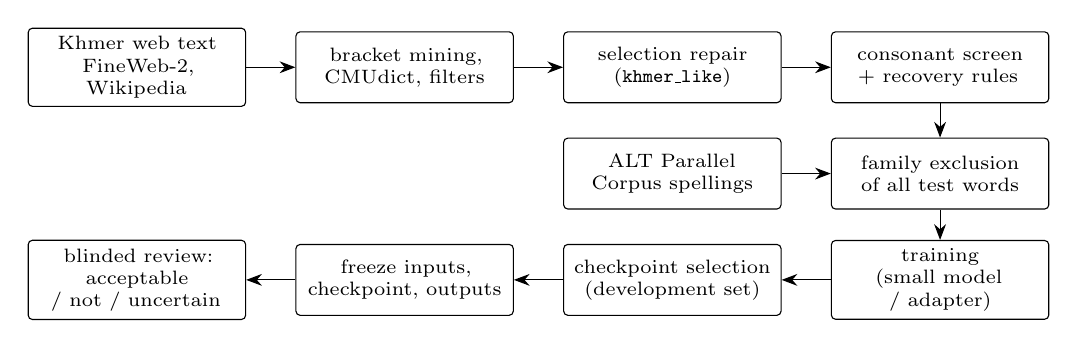
\begin{tikzpicture}[font=\scriptsize,
  box/.style={draw, rounded corners=1.5pt, align=center, inner sep=3pt, minimum height=9mm, text width=2.55cm},
  arr/.style={-{Stealth[length=2mm]}}]
\node[box] (web)    at (0,0)    {Khmer web text\\ FineWeb-2, Wikipedia};
\node[box] (mine)   at (3.4,0)  {bracket mining,\\ CMUdict, filters};
\node[box] (repair) at (6.8,0)  {selection repair\\ (\texttt{khmer\_like})};
\node[box] (screen) at (10.2,0) {consonant screen\\ + recovery rules};
\node[box] (alt)    at (6.8,-1.35) {ALT Parallel\\ Corpus spellings};
\node[box] (fam)    at (10.2,-1.35) {family exclusion\\ of all test words};
\node[box] (train)  at (10.2,-2.7) {training\\ (small model / adapter)};
\node[box] (sel)    at (6.8,-2.7)  {checkpoint selection\\ (development set)};
\node[box] (freeze) at (3.4,-2.7)  {freeze inputs,\\ checkpoint, outputs};
\node[box] (judge)  at (0,-2.7)    {blinded review: acceptable\\ / not / uncertain};
\draw[arr] (web) -- (mine); \draw[arr] (mine) -- (repair); \draw[arr] (repair) -- (screen);
\draw[arr] (screen) -- (fam); \draw[arr] (alt) -- (fam); \draw[arr] (fam) -- (train);
\draw[arr] (train) -- (sel); \draw[arr] (sel) -- (freeze); \draw[arr] (freeze) -- (judge);
\end{tikzpicture}
\caption{Data and evaluation pipeline of the released adapter (ALT spellings pass the same consonant screen). The
small model used the mining and filter steps before the selection repair and was evaluated against reference lists
rather than by blinded review.}
\label{fig:pipeline}
\end{figure}

\section{Notes on the evidence}
\label{app:notes}
{\small
\begin{itemize}
\item Every number in this report is generated from the project's committed result files at revision
  \texttt{d7e7d80} by \texttt{tools/extract.py}; \texttt{EVIDENCE\_LEDGER.md} maps each to its file and field.
  The per-group counts of the first test exist only as a table in its experiment report and were transcribed;
  they sum to the recorded totals.
\item The development review's labels were given in chat and transcribed under four interpretation rules the judge
  confirmed (for example, unnamed candidates of an item are not acceptable). The two blinded tests and the coverage
  diagnostic were clicked directly on the review page. Pooled 60-word percentages in some project notes mix its two samples
  and are not used.
\item The released small model's published latency (17/30\,ms) is from the first of three recorded measurement
  runs; later runs gave \val{s.t2.p50}/\val{s.t2.p95} and \val{s.t3.p50}/\val{s.t3.p95}\,ms (median/95th
  percentile). Table~\ref{tab:releases} gives the range.
\item Parity checks used all 276 development rows and 245 evaluation rows, including items outside the primary
  scoring sets (253 and 228 items).
\end{itemize}
}

\end{document}
